% Graphic for TeX using PGF
% Title: /home/yy12135/MyGit/tinyDTLS-Traffic-Analysis/Writings/First-year-review_20150422/Pics/OddOrEven.dia
% Creator: Dia v0.97.2
% CreationDate: Mon Mar  2 17:12:59 2015
% For: yy12135
% \usepackage{tikz}
% The following commands are not supported in PSTricks at present
% We define them conditionally, so when they are implemented,
% this pgf file will use them.
\ifx\du\undefined
  \newlength{\du}
\fi
\setlength{\du}{15\unitlength}
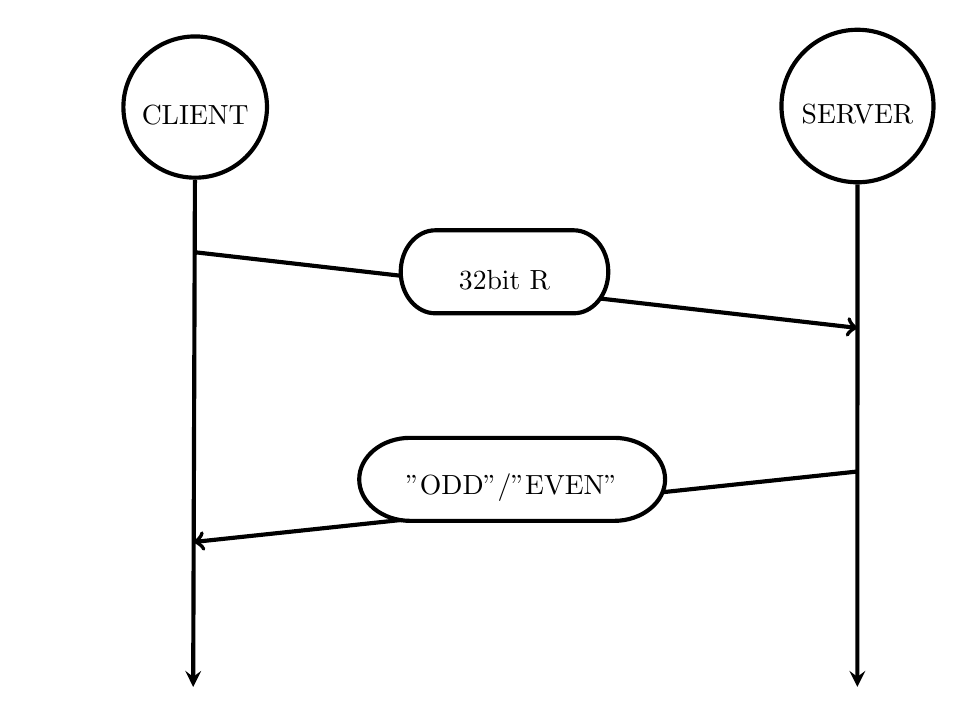
\begin{tikzpicture}
\pgftransformxscale{1.000000}
\pgftransformyscale{-1.000000}
\definecolor{dialinecolor}{rgb}{0.000000, 0.000000, 0.000000}
\pgfsetstrokecolor{dialinecolor}
\definecolor{dialinecolor}{rgb}{1.000000, 1.000000, 1.000000}
\pgfsetfillcolor{dialinecolor}
% setfont left to latex
\definecolor{dialinecolor}{rgb}{0.000000, 0.000000, 0.000000}
\pgfsetstrokecolor{dialinecolor}
\node[anchor=west] at (11.000000\du,9.000000\du){};
\definecolor{dialinecolor}{rgb}{1.000000, 1.000000, 1.000000}
\pgfsetfillcolor{dialinecolor}
\pgfpathellipse{\pgfpoint{31.003315\du}{10.006491\du}}{\pgfpoint{1.831366\du}{0\du}}{\pgfpoint{0\du}{1.837164\du}}
\pgfusepath{fill}
\pgfsetlinewidth{0.100000\du}
\pgfsetdash{}{0pt}
\pgfsetdash{}{0pt}
\pgfsetmiterjoin
\definecolor{dialinecolor}{rgb}{0.000000, 0.000000, 0.000000}
\pgfsetstrokecolor{dialinecolor}
\pgfpathellipse{\pgfpoint{31.003315\du}{10.006491\du}}{\pgfpoint{1.831366\du}{0\du}}{\pgfpoint{0\du}{1.837164\du}}
\pgfusepath{stroke}
% setfont left to latex
\definecolor{dialinecolor}{rgb}{0.000000, 0.000000, 0.000000}
\pgfsetstrokecolor{dialinecolor}
\node at (31.003315\du,10.201491\du){SERVER};
\pgfsetlinewidth{0.100000\du}
\pgfsetdash{}{0pt}
\pgfsetdash{}{0pt}
\pgfsetbuttcap
{
\definecolor{dialinecolor}{rgb}{0.000000, 0.000000, 0.000000}
\pgfsetfillcolor{dialinecolor}
% was here!!!
\pgfsetarrowsend{stealth}
\definecolor{dialinecolor}{rgb}{0.000000, 0.000000, 0.000000}
\pgfsetstrokecolor{dialinecolor}
\draw (31.002868\du,11.893189\du)--(31.000000\du,24.000000\du);
}
\pgfsetlinewidth{0.100000\du}
\pgfsetdash{}{0pt}
\pgfsetdash{}{0pt}
\pgfsetbuttcap
{
\definecolor{dialinecolor}{rgb}{0.000000, 0.000000, 0.000000}
\pgfsetfillcolor{dialinecolor}
% was here!!!
\pgfsetarrowsend{to}
\definecolor{dialinecolor}{rgb}{0.000000, 0.000000, 0.000000}
\pgfsetstrokecolor{dialinecolor}
\draw (15.036382\du,13.528274\du)--(31.002048\du,15.352278\du);
}
\pgfsetlinewidth{0.100000\du}
\pgfsetdash{}{0pt}
\pgfsetdash{}{0pt}
\pgfsetbuttcap
{
\definecolor{dialinecolor}{rgb}{0.000000, 0.000000, 0.000000}
\pgfsetfillcolor{dialinecolor}
% was here!!!
\pgfsetarrowsend{to}
\definecolor{dialinecolor}{rgb}{0.000000, 0.000000, 0.000000}
\pgfsetstrokecolor{dialinecolor}
\draw (31.001229\du,18.811367\du)--(15.012127\du,20.509425\du);
}
\definecolor{dialinecolor}{rgb}{1.000000, 1.000000, 1.000000}
\pgfsetfillcolor{dialinecolor}
\pgfpathellipse{\pgfpoint{15.048531\du}{10.031365\du}}{\pgfpoint{1.729717\du}{0\du}}{\pgfpoint{0\du}{1.701399\du}}
\pgfusepath{fill}
\pgfsetlinewidth{0.100000\du}
\pgfsetdash{}{0pt}
\pgfsetdash{}{0pt}
\pgfsetmiterjoin
\definecolor{dialinecolor}{rgb}{0.000000, 0.000000, 0.000000}
\pgfsetstrokecolor{dialinecolor}
\pgfpathellipse{\pgfpoint{15.048531\du}{10.031365\du}}{\pgfpoint{1.729717\du}{0\du}}{\pgfpoint{0\du}{1.701399\du}}
\pgfusepath{stroke}
% setfont left to latex
\definecolor{dialinecolor}{rgb}{0.000000, 0.000000, 0.000000}
\pgfsetstrokecolor{dialinecolor}
\node at (15.048531\du,10.226365\du){CLIENT};
\pgfsetlinewidth{0.100000\du}
\pgfsetdash{}{0pt}
\pgfsetdash{}{0pt}
\pgfsetbuttcap
{
\definecolor{dialinecolor}{rgb}{0.000000, 0.000000, 0.000000}
\pgfsetfillcolor{dialinecolor}
% was here!!!
\pgfsetarrowsend{stealth}
\definecolor{dialinecolor}{rgb}{0.000000, 0.000000, 0.000000}
\pgfsetstrokecolor{dialinecolor}
\draw (15.042445\du,11.782986\du)--(15.000000\du,24.000000\du);
}
\pgfsetlinewidth{0.100000\du}
\pgfsetdash{}{0pt}
\pgfsetdash{}{0pt}
\pgfsetbuttcap
\pgfsetmiterjoin
\pgfsetlinewidth{0.100000\du}
\pgfsetbuttcap
\pgfsetmiterjoin
\pgfsetdash{}{0pt}
\definecolor{dialinecolor}{rgb}{1.000000, 1.000000, 1.000000}
\pgfsetfillcolor{dialinecolor}
\pgfpathmoveto{\pgfpoint{20.833333\du}{13.000000\du}}
\pgfpathlineto{\pgfpoint{24.166667\du}{13.000000\du}}
\pgfpathcurveto{\pgfpoint{24.626904\du}{13.000000\du}}{\pgfpoint{25.000000\du}{13.447715\du}}{\pgfpoint{25.000000\du}{14.000000\du}}
\pgfpathcurveto{\pgfpoint{25.000000\du}{14.552285\du}}{\pgfpoint{24.626904\du}{15.000000\du}}{\pgfpoint{24.166667\du}{15.000000\du}}
\pgfpathlineto{\pgfpoint{20.833333\du}{15.000000\du}}
\pgfpathcurveto{\pgfpoint{20.373096\du}{15.000000\du}}{\pgfpoint{20.000000\du}{14.552285\du}}{\pgfpoint{20.000000\du}{14.000000\du}}
\pgfpathcurveto{\pgfpoint{20.000000\du}{13.447715\du}}{\pgfpoint{20.373096\du}{13.000000\du}}{\pgfpoint{20.833333\du}{13.000000\du}}
\pgfusepath{fill}
\definecolor{dialinecolor}{rgb}{0.000000, 0.000000, 0.000000}
\pgfsetstrokecolor{dialinecolor}
\pgfpathmoveto{\pgfpoint{20.833333\du}{13.000000\du}}
\pgfpathlineto{\pgfpoint{24.166667\du}{13.000000\du}}
\pgfpathcurveto{\pgfpoint{24.626904\du}{13.000000\du}}{\pgfpoint{25.000000\du}{13.447715\du}}{\pgfpoint{25.000000\du}{14.000000\du}}
\pgfpathcurveto{\pgfpoint{25.000000\du}{14.552285\du}}{\pgfpoint{24.626904\du}{15.000000\du}}{\pgfpoint{24.166667\du}{15.000000\du}}
\pgfpathlineto{\pgfpoint{20.833333\du}{15.000000\du}}
\pgfpathcurveto{\pgfpoint{20.373096\du}{15.000000\du}}{\pgfpoint{20.000000\du}{14.552285\du}}{\pgfpoint{20.000000\du}{14.000000\du}}
\pgfpathcurveto{\pgfpoint{20.000000\du}{13.447715\du}}{\pgfpoint{20.373096\du}{13.000000\du}}{\pgfpoint{20.833333\du}{13.000000\du}}
\pgfusepath{stroke}
% setfont left to latex
\definecolor{dialinecolor}{rgb}{0.000000, 0.000000, 0.000000}
\pgfsetstrokecolor{dialinecolor}
\node at (22.500000\du,14.200000\du){32bit R};
\pgfsetlinewidth{0.100000\du}
\pgfsetdash{}{0pt}
\pgfsetdash{}{0pt}
\pgfsetbuttcap
\pgfsetmiterjoin
\pgfsetlinewidth{0.100000\du}
\pgfsetbuttcap
\pgfsetmiterjoin
\pgfsetdash{}{0pt}
\definecolor{dialinecolor}{rgb}{1.000000, 1.000000, 1.000000}
\pgfsetfillcolor{dialinecolor}
\pgfpathmoveto{\pgfpoint{20.228125\du}{18.000000\du}}
\pgfpathlineto{\pgfpoint{25.140625\du}{18.000000\du}}
\pgfpathcurveto{\pgfpoint{25.818900\du}{18.000000\du}}{\pgfpoint{26.368750\du}{18.447715\du}}{\pgfpoint{26.368750\du}{19.000000\du}}
\pgfpathcurveto{\pgfpoint{26.368750\du}{19.552285\du}}{\pgfpoint{25.818900\du}{20.000000\du}}{\pgfpoint{25.140625\du}{20.000000\du}}
\pgfpathlineto{\pgfpoint{20.228125\du}{20.000000\du}}
\pgfpathcurveto{\pgfpoint{19.549850\du}{20.000000\du}}{\pgfpoint{19.000000\du}{19.552285\du}}{\pgfpoint{19.000000\du}{19.000000\du}}
\pgfpathcurveto{\pgfpoint{19.000000\du}{18.447715\du}}{\pgfpoint{19.549850\du}{18.000000\du}}{\pgfpoint{20.228125\du}{18.000000\du}}
\pgfusepath{fill}
\definecolor{dialinecolor}{rgb}{0.000000, 0.000000, 0.000000}
\pgfsetstrokecolor{dialinecolor}
\pgfpathmoveto{\pgfpoint{20.228125\du}{18.000000\du}}
\pgfpathlineto{\pgfpoint{25.140625\du}{18.000000\du}}
\pgfpathcurveto{\pgfpoint{25.818900\du}{18.000000\du}}{\pgfpoint{26.368750\du}{18.447715\du}}{\pgfpoint{26.368750\du}{19.000000\du}}
\pgfpathcurveto{\pgfpoint{26.368750\du}{19.552285\du}}{\pgfpoint{25.818900\du}{20.000000\du}}{\pgfpoint{25.140625\du}{20.000000\du}}
\pgfpathlineto{\pgfpoint{20.228125\du}{20.000000\du}}
\pgfpathcurveto{\pgfpoint{19.549850\du}{20.000000\du}}{\pgfpoint{19.000000\du}{19.552285\du}}{\pgfpoint{19.000000\du}{19.000000\du}}
\pgfpathcurveto{\pgfpoint{19.000000\du}{18.447715\du}}{\pgfpoint{19.549850\du}{18.000000\du}}{\pgfpoint{20.228125\du}{18.000000\du}}
\pgfusepath{stroke}
% setfont left to latex
\definecolor{dialinecolor}{rgb}{0.000000, 0.000000, 0.000000}
\pgfsetstrokecolor{dialinecolor}
\node at (22.684375\du,19.200000\du){"ODD"/"EVEN"};
\end{tikzpicture}
